\pgfplotsset{every axis/.append style={font=\scriptsize}}
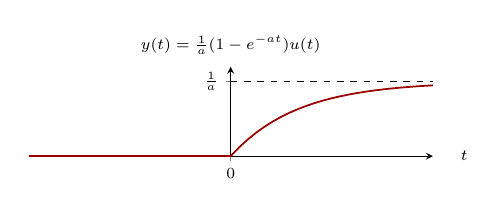
\begin{tikzpicture}[scale=0.8]
\begin{axis}[
	name=axis1,
       width=8cm,
       height=3cm,	
	axis y line=middle,
	axis x line=bottom,
	ymin=0,ymax=1.2,
	xmin=-3,xmax=3,	
	xlabel=$t$,
	ylabel= {$y(t) = \frac{1}{a}(1-e^{-at})u(t)$},	
	xtick={0},
	ytick={1},
	yticklabel={$\frac{1}{a}$},
	every axis x label/.style={at={(ticklabel* cs:1.05)},    anchor=west},
	every axis y label/.style={at={(ticklabel* cs:1.05)},    anchor=south},	
	clip=false,
]
	\addplot [thin, dashed] coordinates {(0,1) (3,1)};
	\addplot [thick, red!60!black] coordinates {(-3,0) (0,0)};
	\addplot [thick, red!60!black, domain=0:3] {1-exp(-x)};
\end{axis}

\end{tikzpicture} 